% Template:     Informe LaTeX
% Documento:    Archivo de ejemplo
% Versión:      8.4.4 (02/12/2025)
% Codificación: UTF-8
%
% Autor: Pablo Pizarro R.
%        pablo@ppizarror.com
%
% Manual template: [https://latex.ppizarror.com/informe]
% Licencia MIT:    [https://opensource.org/licenses/MIT]

% ------------------------------------------------------------------------------
% NUEVA SECCIÓN
% ------------------------------------------------------------------------------
\section{Descripción del proyecto}
El presente trabajo aborda la resolución de un problema de búsqueda de rutas en entornos discretos mediante la implementación de un agente inteligente. Específicamente,
se desarrolló un algoritmo de Búsqueda en Grafo Primero en Profundidad (DFS, por sus siglas en inglés) para encontrar un camino válido desde un punto de inicio hasta
una meta dentro de un laberinto generado de forma procedimental\footnote{El código fuente completo
de la implementación en Python, así como las visualizaciones, se encuentran disponibles en el repositorio:
\url{https://github.com/enriqfl/Navegacion-Autonoma-en-Laberintos}}

% SUB-SECCIÓN
\subsection{Contexto}

El problema se origina en el campo de la Inteligencia Artificial, específicamente en el diseño de agentes racionales y algoritmos de búsqueda no informada. La navegación en laberintos es un problema clásico que sirve como abstracción para situaciones más complejas del mundo real, como la planificación de trayectorias en robótica, el enrutamiento de paquetes en redes de computadoras o la resolución de problemas de logística.

En este contexto, un laberinto representa un entorno estático y determinista donde un agente debe tomar decisiones secuenciales (moverse arriba, abajo, izquierda o derecha) para transitar de un estado inicial a un estado objetivo, evitando obstáculos estructurales (paredes). 

\subsubsection{Visualización}
El entorno se modela como una cuadrícula bidimensional (grid) donde las celdas de espacio libre y las paredes determinan la topología del problema. Gráficamente, el algoritmo de generación crea un patrón de pasillos laberínticos mediante la técnica de "búsqueda en profundidad aleatoria" (Randomized DFS), garantizando que siempre exista al menos un camino posible hacia la meta.

% ------------------------------------------------------------------------------
% PLACEHOLDER DE IMAGEN - REEMPLAZAR RUTA CUANDO COMPILES
% ------------------------------------------------------------------------------
\begin{figure}[htbp]
    \centering
    % NOTA PARA EL USUARIO: Reemplaza 'img/tu_laberinto_aqui.png' con una captura del laberinto generado en tu notebook.
    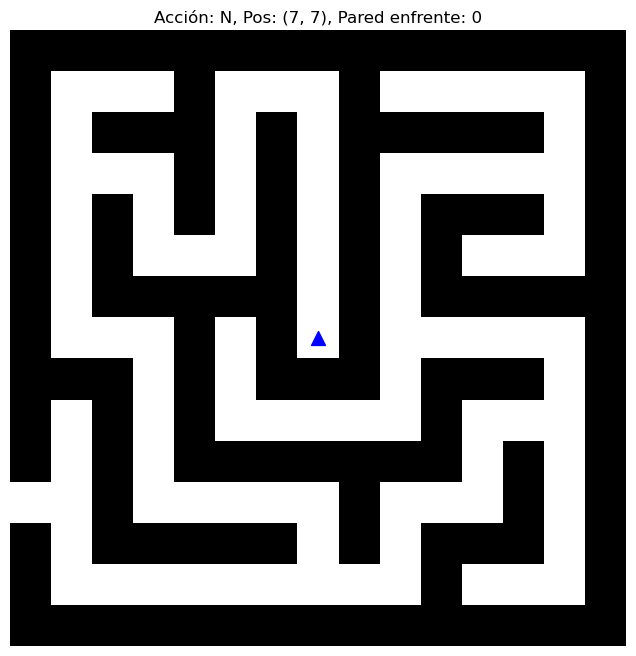
\includegraphics[width=0.6\textwidth]{img/generacion_inicial.png} 
    \caption*{Representación del laberinto generado. Las áreas oscuras representan paredes y el rastro indica la exploración del agente.}
    \label{fig:maze_representation}
\end{figure}

% SUB-SECCIÓN
\subsection{Problema}

Dado un conjunto de datos espaciales representados como una matriz binaria (donde los ceros son caminos libres y los unos son paredes), el problema consiste en determinar una secuencia de acciones direccionales válidas que permitan a un agente transitar desde una coordenada inicial predefinida hasta una coordenada meta.

\subsubsection{Datos de entrada y salida}
\begin{itemize}
    \item \textbf{Entrada:} Una matriz $M$ de tamaño $(2m+1) \times (2n+1)$ representando la topología del laberinto, una tupla de coordenadas de inicio y una tupla de coordenadas meta.
    \item \textbf{Salida:} El algoritmo de búsqueda debe retornar una secuencia (o lista) de acciones discretas (Norte, Sur, Este, Oeste) y los estados (coordenadas) visitados que conforman la ruta solución.
\end{itemize}

% ------------------------------------------------------------------------------
% NUEVA SECCIÓN
% ------------------------------------------------------------------------------
\section{Planteamiento del problema}

% SUB-SECCIÓN
\subsection{Definición de un estado del problema}
Un estado es una estructura de datos que representa la ubicación del agente dentro del entorno en un momento dado. 

Matemáticamente, debido a que el laberinto se mapea sobre una cuadrícula, un estado $E$ se define de manera precisa como una 2-tupla de números enteros que corresponden a los índices de fila y columna de la matriz del entorno:
$$E := (r, c) \text{ con } r, c \in \mathbb{Z}^{+}$$

El planteamiento parte de un estado inicial $E_{0} = (r_{inicio}, c_{inicio})$ situado en el centro geométrico de la matriz, y el objetivo de la búsqueda es alcanzar un estado final $E_{f} = (r_{meta}, c_{meta})$ ubicado en uno de los bordes externos del laberinto.

\subsection{Representación de un estado para el algoritmo de búsqueda}
Para que el agente pueda transitar entre estados y el algoritmo explore el árbol de soluciones, se debe formalizar el modelo de transición. A partir de un estado coordenado $E = (r, c)$, el agente cuenta con un espacio de acciones discreto y constante definido por los puntos cardinales:
$$Acciones := \{'N', 'S', 'E', 'O'\}$$

La función resultado (\textit{Result}), que genera los estados hijos (sucesores), aplica un operador de desplazamiento sumando vectores direccionales al estado actual, siempre y cuando la celda destino no sea una pared (es decir, que el valor en la matriz sea igual a 0). Matemáticamente, el desplazamiento $\Delta(r,c)$ se rige por:
\begin{itemize}
    \item $N \rightarrow \Delta = (-1, 0)$
    \item $S \rightarrow \Delta = (1, 0)$
    \item $E \rightarrow \Delta = (0, 1)$
    \item $O \rightarrow \Delta = (0, -1)$
\end{itemize}

Al evaluar las acciones disponibles en un estado válido, el algoritmo construye iterativamente un árbol de búsqueda (gestionado mediante la clase \texttt{Node}), donde cada nodo encapsula el estado actual, una referencia a su nodo padre y la acción que lo originó.

% ------------------------------------------------------------------------------
% NUEVA SECCIÓN
% ------------------------------------------------------------------------------

\clearpage
\section{Metodología}

La estrategia implementada para solucionar el problema es la \textbf{Búsqueda en Grafo Primero en Profundidad} (\textit{Depth-First Graph Search}). Este algoritmo no informado expande siempre el nodo más profundo en la frontera de búsqueda actual. La metodología se desglosa en los siguientes componentes:

\begin{itemize}
    \item \textbf{Estructura LIFO (Pila):} La frontera de exploración se administra utilizando una estructura de datos tipo Pila (\textit{Stack}). Esto asegura que el último nodo descubierto sea el primero en ser expandido, provocando que el agente siga un camino hasta encontrar un callejón sin salida o la meta.
    
    \item \textbf{Control de estados repetidos (Gráfica):} Para evitar bucles infinitos causados por caminos cíclicos o la reversión inmediata de movimientos (por ejemplo, ir al Norte y luego al Sur repetidamente), se implementó un registro en memoria (conjunto \texttt{visited}). Si un estado ya fue explorado, el algoritmo omite su re-expansión.
    
    \item \textbf{Expansión y Evaluación:} En cada iteración, el agente extrae un nodo de la frontera, lo marca como visitado y verifica si cumple la condición de meta. Si no es la meta, genera todos los estados sucesores válidos (evitando paredes) y los añade a la frontera.
    
    \item \textbf{Construcción del camino:} Una vez que el estado extraído coincide con el estado meta, el algoritmo recupera la ruta óptima encontrada recorriendo recursivamente los nodos desde el objetivo hasta la raíz (estado inicial) utilizando el atributo \texttt{parent} de cada nodo.
\end{itemize}

\section{Resultados}
Al ejecutar el modelo utilizando una dimensión paramétrica de $m=10$ y $n=10$, el algoritmo de búsqueda DFS logró resolver el laberinto de manera determinista. 

\subsection{Comportamiento y análisis visual}
El rastro de solución fue procesado mediante \texttt{matplotlib.animation} para documentar el progreso del agente paso a paso. Se observa cómo el agente toma decisiones basadas en el último nodo disponible, explorando en profundidad cada pasillo antes de hacer un retroceso (\textit{backtracking}) cuando se encuentra de frente con una obstrucción perimetral.

% ------------------------------------------------------------------------------
% PLACEHOLDER DE IMAGEN - REEMPLAZAR RUTA CUANDO COMPILES
% ------------------------------------------------------------------------------
\begin{figure}[htbp]
    \centering
    % NOTA PARA EL USUARIO: Aquí puedes colocar un frame representativo de la animación (laberinto.gif convertido a frame o simplemente una captura del plot final).
    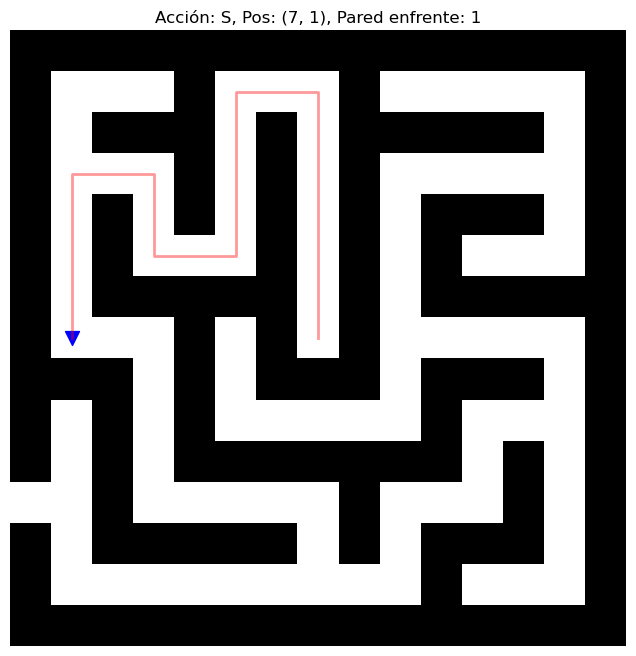
\includegraphics[width=0.45\textwidth]{img/generacion_mitad.png}
    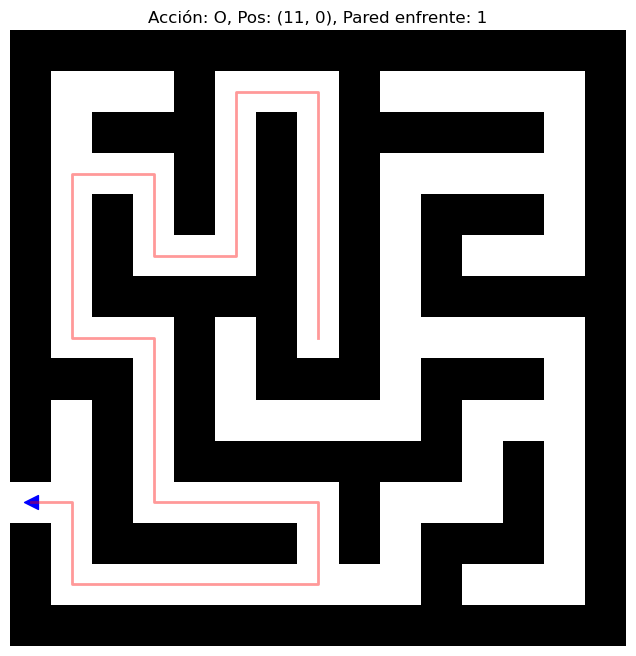
\includegraphics[width=0.45\textwidth]{img/generacion_final.png}
    \caption{A la izquierda: Agente explorando una rama profunda. A la derecha: Agente tras alcanzar con éxito la meta, mostrando la ruta final en rojo.}
    \label{fig:resultados_dfs}
\end{figure}

\clearpage
\section{Conclusiones}

El proyecto demuestra empíricamente la efectividad del algoritmo de Búsqueda Primero en Profundidad adaptado a gráficas para la navegación autónoma en entornos discretos. La integración conjunta de un generador de laberintos garantizó escenarios de prueba válidos, mientras que el control algorítmico mediante conjuntos de memoria (\texttt{visited}) probó ser estrictamente necesario para dotar al agente de racionalidad básica y prevenir colapsos por ciclos de retroalimentación infinita.

Si bien la estrategia DFS garantiza la completitud en espacios de estados finitos (siempre encontrará la salida si existe), se observó que la ruta generada exhibe el comportamiento característico de no optimidad; es decir, el agente no necesariamente toma el camino más corto, sino el primer camino profundo que lo conecte con la meta. Estos hallazgos sientan las bases para iteraciones futuras donde se podrían implementar heurísticas, como en la búsqueda A*, para optimizar el criterio del costo de la trayectoria.

% ------------------------------------------------------------------------------
% REFERENCIAS
% ------------------------------------------------------------------------------
\clearpage
\nocite{*}
\bibliography{library}
